\documentclass{cornouaille}

\begin{document}

\fexo{TS}{Espace : droites, plans et vecteurs}{}



\section{Positions relatives de droites et plans}


	\begin{tikzpicture}[general,y=7.5mm,x=7.5mm]

  \begin{scope}
    \coordinate (1) at (0,0);
    \coordinate (2) at (2,0);
    \coordinate (3) at (2,3);
    \coordinate (4) at (4,3);

    \filldraw [draw=black,fill=A3] (1) -- (2) -- (4) -- (3) -- (1) ;

    \node at (1.5,1.5) {$\times$};
    \node at (1.5,1.5) [above right] {\large $A$};
    \node at (2.2,1.2) {$\times$}; 
    \node at (2.2,1.2) [above right] {\large $B$};
    \node at (2.5,2.2) {$\times$}; 
    \node at (2.5,2.2) [above right] {\large $C$};
  \end{scope}

  \begin{scope}[xshift=2.5cm]
    \coordinate (1) at (0,0);
    \coordinate (2) at (2,0);
    \coordinate (3) at (2,3);
    \coordinate (4) at (4,3);

    \filldraw [draw=black,fill=A3] (1) -- (2) -- (4) -- (3) -- (1) ;

    \draw (1,1) -- (3,2.75) [below] node {\large $d_1$};
    \draw (2,.25) -- (2.2,2.8) node [midway,right] {\large $d_2$};
  \end{scope}

  \begin{scope}[xshift=5cm]
    \coordinate (1) at (0,0);
    \coordinate (2) at (2,0);
    \coordinate (3) at (2,3);
    \coordinate (4) at (4,3);

    \filldraw [draw=black,fill=A3] (1) -- (2) -- (4) -- (3) -- (1) ;

    \draw (1.75,2.25) -- (2.25,.75) node [midway,left] {\large $d$};
    \draw (2,2.5) -- (2.5,1) node [midway,above right] {\large $d'$};
  \end{scope}

\end{tikzpicture}

\begin{rappel}
  \begin{enumerate}
  \item Un plan est défini par :
    \begin{itemize}
    \item [\textbullet] trois points non alignés ou
    \item [\textbullet] deux droites sécantes ou
    \item [\textbullet] deux droites strictement parallèles.
    \end{itemize}
  \item Si un plan $\mathcal{P}$ contient deux points distincts $A$ et
    $ B$ de l'espace,\\
    alors il contient la droite $(AB)$. On note
    $(AB)\subset \mathcal{P}$.
  \item Tous les résultats de géométrie plane (théorèmes de Thalès, de
    Pythagore...)\\ s'appliquent dans chaque plan de l'espace.
  \end{enumerate}
\end{rappel}
Dans la suite du paragraphe, $ABCDEFGH$ est un cube.\\

\begin{proprietes}
[Positions relatives de deux droites]
Deux droites de l'espace sont soit
coplanaires (c'est-à-dire qu'il existe un plan les
contenant toutes les deux), soit non coplanaires (c'est-à-dire qu'il
n'existe aucun plan les contenant toutes les deux).

Si elles sont coplanaires, alors elles sont soit sécantes, soit
parallèles (strictement parallèles ou confondues).
\end{proprietes}

\begin{tabular}{llll}
  \hline
  \multicolumn {3}{|c|}{Droites coplanaires (dans un même plan)} & 
  Droites non coplanaires \tabularnewline \hline \cline{2-4}
  \rowcolor{FondTableaux}Droites sécantes & \multicolumn {2}{c|}{Droites strictement parallèles} & Droites confondues\tabularnewline\hline
 \begin{tikzpicture}[general]

\coordinate (A) at (0,1,1);
\coordinate (B) at (0,0,1);
\coordinate (C) at (1,0,1);
\coordinate (D) at (1,1,1);
\coordinate (E) at (0,1,0);
\coordinate (F) at (0,0,0);
\coordinate (G) at (1,0,0);
\coordinate (H) at (1,1,0);

% \draw [J2,dashed] (A) -- (F);
\draw [dashed,J2] (A) -- (F) -- (.35,-.5,0);
\draw [J1] (-.3,1.5,1) -- (A);
% \draw [J1] (F) -- (.35,-.5);

\draw [dashed,J2] (E)--(F);
\draw [dashed,J2] (F)--(G);
\draw [dashed,J2] (B)--(F);
\draw (E)--(H)--(G); % face arrière
\draw (A)--(B)--(C)--(D)--cycle; % face avant
% arêtes horizontales, de l’arrière vers l’avant
\draw (B) -- (A); % bas gauche
\draw (C) -- (G); % bas droit
\draw (D) -- (H); % haut droit
\draw (A) -- (E); % haut gauche

\node at (A) [left] {$A$};
\node at (B) [below left] {$B$};
\node at (C) [below] {$C$};
\node at (D) [right] {$D$};
\node at (E) [above] {$E$};
\node at (F) [above right] {$F$};
\node at (G) [right] {$G$};
\node at (H) [above right] {$H$};

\node at (.25,-1.25) {\parbox{3cm}{\scriptsize (AD) et (AF) sont sécantes en A}};

\end{tikzpicture} & 
 \begin{tikzpicture}[general]

\coordinate (A) at (0,1,1);
\coordinate (B) at (0,0,1);
\coordinate (C) at (1,0,1);
\coordinate (D) at (1,1,1);
\coordinate (E) at (0,1,0);
\coordinate (F) at (0,0,0);
\coordinate (G) at (1,0,0);
\coordinate (H) at (1,1,0);

\draw [dashed,J2] (E)--(F);
\draw [dashed,J2] (F)--(G);
\draw [dashed,J2] (B)--(F);
\draw (E)--(H)--(G); % face arrière
\draw (A)--(B)--(C)--(D)--cycle; % face avant
% arêtes horizontales, de l’arrière vers l’avant
\draw (B) -- (A); % bas gauche
\draw (C) -- (G); % bas droit
\draw (D) -- (H); % haut droit
\draw (A) -- (E); % haut gauche

\draw [J1] (-1,.75,1) -- (2,1.25,0) node [midway,above] {$I$} node [midway] {$\bullet$};

\node at (A) [left] {$A$};
\node at (B) [below left] {$B$};
\node at (C) [below] {$C$};
\node at (D) [right] {$D$};
\node at (E) [above] {$E$};
\node at (F) [above right] {$F$};
\node at (G) [right] {$G$};
\node at (H) [above right] {$H$};

\node at (.25,-1.25) {\parbox{3cm}{\scriptsize I centre de ADHE (AH) et (AI) sont confondues}};

\end{tikzpicture} & 
 \begin{tikzpicture}[general]

\coordinate (A) at (0,1,1);
\coordinate (B) at (0,0,1);
\coordinate (C) at (1,0,1);
\coordinate (D) at (1,1,1);
\coordinate (E) at (0,1,0);
\coordinate (F) at (0,0,0);
\coordinate (G) at (1,0,0);
\coordinate (H) at (1,1,0);

\draw [dashed,J2] (E)--(F);
\draw [dashed,J2] (F)--(G);
\draw [dashed,J2] (B)--(F);
\draw (E)--(H)--(G); % face arrière
\draw (A)--(B)--(C)--(D)--cycle; % face avant
% arêtes horizontales, de l’arrière vers l’avant
\draw (B) -- (A); % bas gauche
\draw (C) -- (G); % bas droit
\draw (D) -- (H); % haut droit
\draw (A) -- (E); % haut gauche

\draw [J1] (-1,0,0) -- (F);
\draw [J1] (G) -- (1.62,0,0);

\node at (A) [left] {$A$};
\node at (B) [below left] {$B$};
\node at (C) [below] {$C$};
\node at (D) [right] {$D$};
\node at (E) [above] {$E$};
\node at (F) [above right] {$F$};
\node at (G) [right] {$G$};
\node at (H) [above right] {$H$};

\node at (0,-1.25) {\parbox{3cm}{\scriptsize (AD) et (FG) sont strictement parallèles\par}};

\end{tikzpicture} &
 \begin{tikzpicture}[general]

\coordinate (A) at (0,1,1);
\coordinate (B) at (0,0,1);
\coordinate (C) at (1,0,1);
\coordinate (D) at (1,1,1);
\coordinate (E) at (0,1,0);
\coordinate (F) at (0,0,0);
\coordinate (G) at (1,0,0);
\coordinate (H) at (1,1,0);

\draw [dashed,J2] (E)--(F);
\draw [dashed,J2] (F)--(G);
\draw [dashed,J2] (B)--(F);
\draw (E)--(H)--(G); % face arrière
\draw (A)--(B)--(C)--(D)--cycle; % face avant
% arêtes horizontales, de l’arrière vers l’avant
\draw (B) -- (A); % bas gauche
\draw (C) -- (G); % bas droit
\draw (D) -- (H); % haut droit
\draw (A) -- (E); % haut gauche

\draw [J1] (-1,0,1) -- (2,0,1);
\draw [dashed,J2] (A) -- (F) -- (.4,-.5,0);
\draw [J1] (-.33,1.5,1) -- (A);

\node at (A) [left] {$A$};
\node at (B) [below left] {$B$};
\node at (C) [below] {$C$};
\node at (D) [right] {$D$};
\node at (E) [above] {$E$};
\node at (F) [above right] {$F$};
\node at (G) [right] {$G$};
\node at (H) [above right] {$H$};

\node at (0,-1.25) {\parbox{3cm}{\scriptsize (BC) et (AF) sont non\par coplanaires\par}};

\end{tikzpicture}
\end{tabular}

\begin{proprietes}[Positions relatives de deux plans]
Deux plans de l'espace sont soit sécants (leur intersection est une
droite), soit parallèles.
\end{proprietes}

\begin{tabular}{lll}
  \hline
  \multicolumn {1}{|c|}{Plans sécants} & \multicolumn {2}{c|}{Plans parallèles} \tabularnewline\hline
  \begin{tikzpicture}[general]

\coordinate (A) at (0,1,1);
\coordinate (B) at (0,0,1);
\coordinate (C) at (1,0,1);
\coordinate (D) at (1,1,1);
\coordinate (E) at (0,1,0);
\coordinate (F) at (0,0,0);
\coordinate (G) at (1,0,0);
\coordinate (H) at (1,1,0);

\draw [dashed,J2] (E)--(F);
\draw [dashed,J2] (F)--(G);
\draw [dashed,J2] (B)--(F);
\draw (E)--(H)--(G); % face arrière
\draw (A)--(B)--(C)--(D)--cycle; % face avant
% arêtes horizontales, de l’arrière vers l’avant
\draw (B) -- (A); % bas gauche
\draw (C) -- (G); % bas droit
\draw (D) -- (H); % haut droit
\draw (A) -- (E); % haut gauche

\fill [J2,opacity=.2] (A) -- (D) -- (H) -- (E) -- (A);
\fill [J2,opacity=.2] (D) -- (H) -- (G) -- (C);

\tkzDefPoint(0,0){X};
\tkzDefPoint(1.5,1.5){Z};
\tkzDrawLine [color=J1, add=.1 and .1](X,Z);

\node at (A) [left] {$A$};
\node at (B) [below left] {$B$};
\node at (C) [below] {$C$};
\node at (D) [right] {$D$};
\node at (E) [above] {$E$};
\node at (F) [above right] {$F$};
\node at (G) [right] {$G$};
\node at (H) [above right] {$H$};

\node at (.25,-1.25) {\parbox{5cm}{\scriptsize Les plans (CGH) et (ADH) sont sécants
  selon la droite (DH)}};

\end{tikzpicture} & 
  \begin{tikzpicture}[general]

\coordinate (A) at (0,1,1);
\coordinate (B) at (0,0,1);
\coordinate (C) at (1,0,1);
\coordinate (D) at (1,1,1);
\coordinate (E) at (0,1,0);
\coordinate (F) at (0,0,0);
\coordinate (G) at (1,0,0);
\coordinate (H) at (1,1,0);

\draw [dashed,J2] (E)--(F);
\draw [dashed,J2] (F)--(G);
\draw [dashed,J2] (B)--(F);
\draw (E)--(H)--(G); % face arrière
\draw (A)--(B)--(C)--(D)--cycle; % face avant
% arêtes horizontales, de l’arrière vers l’avant
\draw (B) -- (A); % bas gauche
\draw (C) -- (G); % bas droit
\draw (D) -- (H); % haut droit
\draw (A) -- (E); % haut gauche

\fill [J2,opacity=.2] (A) -- (D) -- (H) -- (E) -- (A);
\fill [J2,opacity=.2] (B) -- (C) -- (G) -- (F);

\node at (A) [left] {$A$};
\node at (B) [below left] {$B$};
\node at (C) [below] {$C$};
\node at (D) [right] {$D$};
\node at (E) [above] {$E$};
\node at (F) [above right] {$F$};
\node at (G) [right] {$G$};
\node at (H) [above right] {$H$};

\node at (.25,-1.25) {\parbox{5cm}{\scriptsize Les plans (BCG) et (ADH) sont strictement\\ parallèles}};

\end{tikzpicture} &  
 \begin{tikzpicture}[general]

\coordinate (A) at (0,1,1);
\coordinate (B) at (0,0,1);
\coordinate (C) at (1,0,1);
\coordinate (D) at (1,1,1);
\coordinate (E) at (0,1,0);
\coordinate (F) at (0,0,0);
\coordinate (G) at (1,0,0);
\coordinate (H) at (1,1,0);

\draw [dashed,J2] (E)--(F);
\draw [dashed,J2] (F)--(G);
\draw [dashed,J2] (B)--(F);
\draw (E)--(H)--(G); % face arrière
\draw (A)--(B)--(C)--(D)--cycle; % face avant
% arêtes horizontales, de l’arrière vers l’avant
\draw (B) -- (A); % bas gauche
\draw (C) -- (G); % bas droit
\draw (D) -- (H); % haut droit
\draw (A) -- (E); % haut gauche

\fill [J2,opacity=.2] (A) -- (D) -- (H) -- (E) -- (A);

\node at (A) [left] {$A$};
\node at (B) [below left] {$B$};
\node at (C) [below] {$C$};
\node at (D) [right] {$D$};
\node at (E) [above] {$E$};
\node at (F) [above right] {$F$};
\node at (G) [right] {$G$};
\node at (H) [above right] {$H$};

\node at (.25,-1.25) {\parbox{5cm}{\scriptsize Les plans (EAD) et
    (ADH) sont confondus}};

\end{tikzpicture}\tabularnewline\hline
\end{tabular}



\begin{proprietes}[Positions relatives d'une droite et d'un plan]
  Une droite et un plan de l'espace sont soit sécants, soit parallèles.
\end{proprietes}

\begin{tabular}{llll}
  \hline
  \multicolumn {1}{|c|}{Droite et plan sécants} & 
  \multicolumn{2}{c|}{Droite et plan parallèles} \tabularnewline\hline
  \begin{tikzpicture}[general]

\coordinate (A) at (0,1,1);
\coordinate (B) at (0,0,1);
\coordinate (C) at (1,0,1);
\coordinate (D) at (1,1,1);
\coordinate (E) at (0,1,0);
\coordinate (F) at (0,0,0);
\coordinate (G) at (1,0,0);
\coordinate (H) at (1,1,0);

\draw [dashed,J2] (E)--(F);
\draw [dashed,J2] (F)--(G);
\draw [dashed,J2] (B)--(F);
\draw (E)--(H)--(G); % face arrière
\draw (A)--(B)--(C)--(D)--cycle; % face avant
% arêtes horizontales, de l’arrière vers l’avant
\draw (B) -- (A); % bas gauche
\draw (C) -- (G); % bas droit
\draw (D) -- (H); % haut droit
\draw (A) -- (E); % haut gauche

\draw [J1] (-1,.75,1) -- (2,1.25,0);

\fill [J2,opacity=.2] (D)--(C)--(G)--(H);

\node at (A) [left] {$A$};
\node at (B) [below left] {$B$};
\node at (C) [below] {$C$};
\node at (D) [right] {$D$};
\node at (E) [above] {$E$};
\node at (F) [above right] {$F$};
\node at (G) [right] {$G$};
\node at (H) [above right] {$H$};

\node at (.25,-1.25) {\parbox{5cm}{\scriptsize La droite (AH) est sécante en H au plan (DCG)}};

\end{tikzpicture} & 
  \begin{tikzpicture}[general]

\coordinate (A) at (0,1,1);
\coordinate (B) at (0,0,1);
\coordinate (C) at (1,0,1);
\coordinate (D) at (1,1,1);
\coordinate (E) at (0,1,0);
\coordinate (F) at (0,0,0);
\coordinate (G) at (1,0,0);
\coordinate (H) at (1,1,0);

\draw [dashed,J2] (E)--(F);
\draw [dashed,J2] (F)--(G);
\draw [dashed,J2] (B)--(F);
\draw (E)--(H)--(G); % face arrière
\draw (A)--(B)--(C)--(D)--cycle; % face avant
% arêtes horizontales, de l’arrière vers l’avant
\draw (B) -- (A); % bas gauche
\draw (C) -- (G); % bas droit
\draw (D) -- (H); % haut droit
\draw (A) -- (E); % haut gauche

\draw [J1] (-1,.75,1) -- (2,1.25,0);

\fill [J2,opacity=.2] (B)--(C)--(G)--(F);

\node at (A) [left] {$A$};
\node at (B) [below left] {$B$};
\node at (C) [below] {$C$};
\node at (D) [right] {$D$};
\node at (E) [above] {$E$};
\node at (F) [above right] {$F$};
\node at (G) [right] {$G$};
\node at (H) [above right] {$H$};

\node at (.25,-1.25) {\parbox{5cm}{\scriptsize La droite (AH) est strictement parallèle
  au plan (BCG)}};

\end{tikzpicture} &  
  
  \begin{tikzpicture}[general]

\coordinate (A) at (0,1,1);
\coordinate (B) at (0,0,1);
\coordinate (C) at (1,0,1);
\coordinate (D) at (1,1,1);
\coordinate (E) at (0,1,0);
\coordinate (F) at (0,0,0);
\coordinate (G) at (1,0,0);
\coordinate (H) at (1,1,0);

\draw [dashed,J2] (E)--(F);
\draw [dashed,J2] (F)--(G);
\draw [dashed,J2] (B)--(F);
\draw (E)--(H)--(G); % face arrière
\draw (A)--(B)--(C)--(D)--cycle; % face avant
% arêtes horizontales, de l’arrière vers l’avant
\draw (B) -- (A); % bas gauche
\draw (C) -- (G); % bas droit
\draw (D) -- (H); % haut droit
\draw (A) -- (E); % haut gauche

\draw [J1] (-1,.75,1) -- (2,1.25,0) node [midway, above] {$I$} node
[midway] {$\bullet$};

\fill [J2,opacity=.2] (A)--(D)--(H)--(E);

\node at (A) [left] {$A$};
\node at (B) [below left] {$B$};
\node at (C) [below] {$C$};
\node at (D) [right] {$D$};
\node at (E) [above] {$E$};
\node at (F) [above right] {$F$};
\node at (G) [right] {$G$};
\node at (H) [above right] {$H$};

\node at (.25,-1.25) {\parbox{4cm}{\scriptsize % $I$ centre de ADHE et
(AH) est contenue dans le plan $(ADH)$}};

\end{tikzpicture}\tabularnewline
  \hline
\end{tabular}

\section{Parallélisme dans l'espace}

\begin{propriete}
  \begin{itemize}
  \item Si deux droites sont parallèles à une même droite alors elles
    sont parallèles entre elles.
  \item Si deux plans sont parallèles à un même plan alors ils sont
    parallèles entre eux.
  \end{itemize}
\end{propriete}
           
\begin{propriete}
  Une droite est parallèle à un plan si et seulement si elle est
  parallèle à une droite de ce plan.
\end{propriete}

\begin{exemple}~\par
  \begin{minipage}{.45\linewidth}
    $d$ est parallèle à $d_1$ et $d_1$ est contenue dans le plan $\wp$
    donc $d$ est parallèle à $\wp$.
  \end{minipage}
  \hfill
  \begin{minipage}{.45\linewidth}
    \begin{tikzpicture}[general]

\fill [A3] (0,0)--(1,0)--(2,2.5)--(1,2.5);
\draw  (0.2,.2)--(1.7,2) node [midway, right] {$d_1$};
\node at (0,0) [above right,xshift=2mm] {$\wp$};
\draw  (-1,1.2)--(.5,3) node [midway,left] {$d$};
\end{tikzpicture}
  \end{minipage}
\end{exemple}

\begin{propriete}
  Si un plan $\wp$ contient deux droites sécantes respectivement
  parallèles à deux droites sécantes d' un plan $\wp'$ alors les plans
  $\wp$ et $\wp'$ sont parallèles.
\end{propriete}
          
\begin{exemple}~\par
  \begin{minipage}{.45\linewidth}
    $d_1$ et $d_2$ sont deux droites du plan $\wp$ ; $d_1$ et $d_2$
    sont sécantes et respectivement parallèles à deux droites du plan
    $\wp'$ donc les plans $\wp$ et $\wp'$ sont parallèles.
  \end{minipage}
  \hfill
  \begin{minipage}{.45\linewidth}
    \begin{tikzpicture}[general]

  \begin{scope}
    \fill [B3] (0,0)--(1,0)--(2,2)--(1,2);
    \draw (0.2,.2)--(1.7,1.8) node [midway, right] {$d_1$};
    \node at (0,0) [above right,xshift=2mm] {$\wp$};
    \draw (1,.2)--(.8,1.5) node [near end,above right,xshift=-1mm] {$d_2$};
  \end{scope}

  \begin{scope}[yshift=-2cm]
    \fill [A3] (0,0)--(1,0)--(2,2)--(1,2);
    \draw (0.2,.2)--(1.7,1.8) node [midway, right] {$d'_1$};
    \node at (0,0) [above right,xshift=2mm] {$\wp'$};
    \draw (1,.2)--(.8,1.5) node [near end,above right,xshift=-1mm] {$d'_2$};
  \end{scope}

\end{tikzpicture}
  \end{minipage}
\end{exemple}

\begin{propriete}
  Si deux plans sont parallèles, alors tout plan qui coupe l'un coupe
  l'autre et les droites d'intersection sont parallèles entre elles.
\end{propriete}

\begin{exemple}~\par
  \begin{minipage}{.45\linewidth}
    Les plans $\wp$ et $\wp'$ sont parallèles et $\wp$ et $\wp''$ sont
    sécants avec $\wp\cap\wp''=d$, donc $\wp'$ et $\wp''$ sont sécants
    et $\wp'\cap\wp''=d'$ où $d'$ est une droite parallèle à $d$.
  \end{minipage}
  \hfill
  \begin{minipage}{.45\linewidth}
   \begin{tikzpicture}[general]

  \filldraw [fill=H3,draw=black] (-.75,0) rectangle (2.75,3);
  \begin{scope}
    \tkzDefPoint(-.5,1.5){A}
    \tkzDefPoint(1.5,1.7){B} 
    \tkzDefPoint(2.5,2.5){C}
    \tkzDefPointWith[colinear= at C](B,A)
    \tkzGetPoint{D}
    \tkzDrawPolygon[color=black,fill=B3](A,B,C,D)
  \end{scope}

  \begin{scope}[yshift=-1cm]
    \tkzDefPoint(-.5,1.5){A}
    \tkzDefPoint(1.5,1.7){B} 
    \tkzDefPoint(2.5,2.5){C}
    \tkzDefPointWith[colinear= at C](B,A)
    \tkzGetPoint{D}
  \end{scope}
  \tkzDrawPolygon[color=black,fill=A3](A,B,C,D)
  \draw (-0.2,2)--(2.2,2) node [near start,below] {$d$};
  \draw (-0.2,1)--(2.2,1) node [near start,below] {$d'$};
  \node at (1.7,.25) {$\wp''$};
  \node at (1.7,1.25) {$\wp'$};
  \node at (1.7,2.25) {$\wp$};
\end{tikzpicture}
  \end{minipage}
\end{exemple}

\begin{propriete} [Théorème du toit]
  \begin{minipage}{.45\linewidth}
    Soit $\wp$ et $\wp'$ deux plans distincts, sécants selon une
    droite $\Delta$.

    Si une droite $d$ de $\wp$ est strictement parallèle à une droite
    $d'$ de $\wp'$ alors la droite $\Delta$ intersection de $\wp$ et
    $\wp'$ est parallèle à $d$ et à $d'$.
  \end{minipage}
  \hfill
  \begin{minipage}{.45\linewidth}
    \begin{tikzpicture}[general]


 \begin{scope}
    \tkzDefPoint(2,.6){A}
    \tkzDefPoint(4,1){B} 
    \tkzDefPoint(3,3.8){C}
    \tkzDefPointWith[colinear= at C](B,A)
    \tkzGetPoint{D}
    \tkzDrawPolygon[color=black,fill=A3](A,B,C,D)
  \end{scope}
 \begin{scope}
    \tkzDefPoint(0,1.2){A}
    \tkzDefPoint(2,1.6){B} 
    \tkzDefPoint(3,3.8){C}
    \tkzDefPointWith[colinear= at C](B,A)
    \tkzGetPoint{D}
    \tkzDrawPolygon[color=black,fill=H3](A,B,C,D)
  \end{scope}

  \draw (-1,3)--(4,4) node [near start,above left] {$\Delta$};
  \draw (-1,1)--(4,2) node [near start,below left] {$d$};
  \draw (-1,0)--(4,1) node [midway,below left] {$d'$};

  \node at (.6,1.75) {$\wp$};
  \node at (2.2,1) {$\wp'$};
 \end{tikzpicture}
  \end{minipage}
\end{propriete}

\begin{preuve}
  Par hypothèse, $\wp\cap\wp'=\Delta$ et $d//d'$. Les droites $d$ et
  $d'$ sont parallèles donc elles sont coplanaires. Donc, il existe un
  plan $Q$ qui contient à la fois $d$ et $d'$. Mais alors $d$ et
  $\Delta$ sont contenues dans $\wp$ et $d'$ et $\Delta$ sont
  contenues dans $\wp'$. Donc : $\wp\cap Q=d$ et $\wp'\cap Q=d'$.

  Montrons que $d//\Delta$.
  Supposons que $d$ et $\Delta$ ne soient pas parallèles. Donc elles
  sont sécantes en un point $A$.

  $A\in d$ et $A\in\Delta$.
  \begin{itemize}
  \item $A\in d$ et $d=\wp\cap Q$ donc $A\in Q$.
  \item $A\in\Delta$ et $\Delta=\wp\cap\wp'$ donc $A\in\wp'$.  D'où
    $A\in Q\cap\wp'=d'$.
  \end{itemize}

  Par conséquent, $A\in d'$ et $A\in d$ et par conséquent, $d$ et $d'$
  sont sécantes en A.
  Ce qui est absurde, contraire à notre hypothèse.

  Les droites $d$ et $\Delta$ sont donc parallèles.  De plus, comme
  $d$ et $d'$ sont parallèles, on en déduit que les droites $d'$ et
  $\Delta$ sont aussi parallèles.  

  \textbf{Conclusion :} L'intersection de $\wp$ et $\wp'$ est une
  droite $\Delta$ parallèle à la fois à $d$ et à $d'$.
\end{preuve}





\begin{methode}[Construire la section d'un solide par  un plan]
  Il s'agit de construire l'intersection de ce plan avec chacune des
  faces du solide.

  

\textbf{Exercice:}



  On considère le cube $ABCDEFGH$ ci-contre.  On note $M$ le milieu du
  segment $[EH]$ et $N$ celui de $[FC]$.

  \begin{tikzpicture}[general]

\coordinate (A) at (0,0,2);
\coordinate (B) at (2,0,2);
\coordinate (F) at (2,2,2);
\coordinate (E) at (0,2,2);
\coordinate (D) at (0,0,0);
\coordinate (C) at (2,0,0);
\coordinate (G) at (2,2,0);
\coordinate (H) at (0,2,0);

\draw [opacity=0] (B)--(G) node [B2,midway,above right,opacity=1,xshift=-1mm] {$N$} node [midway,B2,opacity=1] {+};
\draw [dashed,J2] (A)--(D)--(C);
\draw [dashed,J2] (D)--(H);
\draw (E)--(F)--(G)--(H)--(E) node [B2, midway, above left] {$M
$} node [B2, midway] {+}; % face arrière
\draw (A)--(B)--(C); % face avant
% arêtes horizontales, de l’arrière vers l’avant
\draw (B) -- (A); % bas gauche
\draw (C) -- (G); % bas droit
\draw (F) -- (B); % haut droit
\draw (A) -- (E); % haut gauche


\node at (A) [left] {$A$};
\node at (B) [right] {$B$};
\node at (C) [right] {$C$};
\node at (D) [above right] {$D$};
\node at (E) [left] {$E$};
\node at (F) [right] {$F$};
\node at (G) [above] {$G$};
\node at (H) [above] {$H$};

\end{tikzpicture}

  Tracer la section de ce cube par le plan $(MNG)$.

  

\textbf{Correction}



  L'intersection du plan $(MNG)$ avec la face $HEFG$ est le segment
  $[MG]$. Il est visible, on le trace donc en trait plein.

  $G, N$ et $B$ sont alignés, donc l'intersection du plan $(MNG)$ avec
  la face $FGCB$ est le segment $[GB]$. Il est visible, on le trace
  donc\\ en trait plein.

  \begin{tikzpicture}[general]

\coordinate (A) at (0,0,2);
\coordinate (B) at (2,0,2);
\coordinate (F) at (2,2,2);
\coordinate (E) at (0,2,2);
\coordinate (P) at (0,1,2);
\coordinate (M) at (.4,2.4,2);
\coordinate (N) at (2.2,1.5,2);
\coordinate (D) at (0,0,0);
\coordinate (C) at (2,0,0);
\coordinate (G) at (2,2,0);
\coordinate (H) at (0,2,0);

\filldraw [fill=B2] (G) -- (M) -- (P) -- (B) -- (G);
\draw [opacity=0] (B)--(G) node [B2,midway,above right,opacity=1,xshift=-1mm] {$N$} node [midway,B2,opacity=1] {+};
\draw [dashed,J2] (A)--(D)--(C);
\draw [dashed,J2] (D)--(H);
\draw (E)--(F)--(G)--(H)--(E) node [B2, midway, above left] {$M
$} node [B2, midway] {+}; % face arrière
\draw (A)--(B)--(C); % face avant
% arêtes horizontales, de l’arrière vers l’avant
\draw (B) -- (A); % bas gauche
\draw (C) -- (G); % bas droit
\draw (F) -- (B); % haut droit
\draw (A) -- (E); % haut gauche

\node at (A) [below] {$A$};
\node at (B) [below] {$B$};
\node at (C) [right] {$C$};
\node at (D) [above right] {$D$};
\node at (E) [left] {$E$};
\node at (F) [right] {$F$};
\node at (G) [above] {$G$};
\node at (H) [above] {$H$};
\node at (P) [B2,left] {$P$};

\begin{scope}[xshift=.25mm]
  \tkzDefPoint(-1,-.5){X};
\tkzDefPoint(-.15,2.5){Z};
\tkzDrawLine [color=B2, add=.1 and .1](X,Z);
\end{scope}

\draw [dashed,J2] (M)--(P);

\end{tikzpicture}

  Les faces $EHDA$ et $FGCB$ étant parallèles, l'intersection du plan
  $(MNG)$ avec la face $EHDA$ est le segment passant par $M$ et
  parallèle à $(GN)$. Il n'est pas visible, on le trace donc en
  pointillés.

  Notons $P$ le point d'intersection de $(MNG)$ et
  $(EA)$. L'intersection du plan $(MNG)$ avec la face $ABFE$ est le
  segment $[PB]$. Il est visible, on le trace donc en trait plein.

  La section du cube par le plan $(MNG)$ est le polygone $MGBP$
  colorié en rouge. Comme $(MP)//(GB)$, il s'agit d'un trapèze.
\end{methode}

\section{Orthogonalité dans l'espace}

  Droites orthogonales

\begin{definition}[Orthogonalité de deux droites]
  Deux droites sont orthogonales si leurs parallèles passant par un
  même point sont perpendiculaires dans le plan qu'elles définissent.
\end{definition}

\begin{remarque}
  Deux droites perpendiculaires sont orthogonales mais la réciproque
  est fausse.
\end{remarque}

\begin{exemple}~\par
  \begin{minipage}{.45\linewidth}
    Dans le cube $ABCDEFGH$ ci-contre, $(EF)//(HG)$ et
    $(HG)\perp (GC)$ donc $(EF)$ et $(GC)$ sont orthogonales. On note
    $(EF)\perp (GC)$.
  \end{minipage}
  \hfill
  \begin{minipage}{.45\linewidth}
    \begin{tikzpicture}[general]

\coordinate (A) at (0,0,2);
\coordinate (B) at (2,0,2);
\coordinate (F) at (2,2,2);
\coordinate (E) at (0,2,2);
\coordinate (D) at (0,0,0);
\coordinate (C) at (2,0,0);
\coordinate (G) at (2,2,0);
\coordinate (H) at (0,2,0);

\draw [B2] (-1,2,2)--(E);
\draw [B2] (F)--(3,2,2);
\draw [B2] (G)--(2,3,0);
\draw [B2] (C)--(2,-1,0);
\draw [dashed,J2] (A)--(D)--(C);
\draw [dashed,J2] (D)--(H);
\draw (E)--(F)--(G)--(H)--(E); % face arrière
\draw (A)--(B)--(C); % face avant
% arêtes horizontales, de l’arrière vers l’avant
\draw (B) -- (A); % bas gauche
\draw (C) -- (G); % bas droit
\draw (F) -- (B); % haut droit
\draw (A) -- (E); % haut gauche


\node at (A) [left] {$A$};
\node at (B) [right] {$B$};
\node at (C) [right] {$C$};
\node at (D) [above right] {$D$};
\node at (E) [above left] {$E$};
\node at (F) [above left] {$F$};
\node at (G) [above right] {$G$};
\node at (H) [above] {$H$};

\end{tikzpicture}
  \end{minipage}
\end{exemple}



\begin{definition}[Orthogonalité d’une droite et d’un plan]
  Une droite est orthogonale à un plan lorsqu'elle est orthogonale à
  toutes les droites de ce plan.
\end{definition}
       
\begin{theoreme}
  Si une droite est orthogonale à deux droites sécantes d'un plan
  alors elle est orthogonale à ce plan.
\end{theoreme}

\begin{methode}[Démontrer l'orthogonalité de deux droites]

  

\textbf{Exercice:}



  Dans le cube $ABCDEFGH$ représenté dans l'exemple précédent,
  démontrer que $(GC)\perp (BD)$.

  

\textbf{Correction}



  La droite $(GC)$ est perpendiculaire à $(BC)$ et à $(CD)$ qui sont
  deux droites sécantes du plan $(ABC)$ donc $(GC)$ est orthogonale au
  plan $(ABC)$ donc à toutes les droites de ce plan. En particulier,
  on en déduit que $(GC)\perp (BD)$.
\end{methode}

\section{Vecteurs de l'espace}

\begin{remarque}
  On étend à l'espace la définition et les propriétés des
  vecteurs étudiées dans le plan.
\end{remarque}

\begin{proprietes}[Vecteurs colinéaires]
  Deux vecteurs non nuls $\vec{u}$ et $\vec{v}$ sont colinéaires si et
  seulement si il existe un réel $k$ tel que $\vec{v}=k \vec{u}$.  Par
  convention, le vecteur nul est colinéaire à tout vecteur de
  l'espace.
\end{proprietes}

\begin{propriete}[Caractéristique]
  $A$ et  $B$ étant deux points distincts de l'espace, la droite
  $(AB)$ est l'ensemble des points $M$ de l'espace tels que
  $\overrightarrow{AB}$ et $\overrightarrow{AM}$ soient colinéaires.

  On dit que $\overrightarrow{AB}$ est un vecteur directeur de la
  droite $(AB)$.
\end{propriete}

\begin{definition}[Vecteurs coplanaires]
  Trois vecteurs non nuls $\vec{u}$, $\vec{v}$ et $\vec{w}$ sont
  coplanaires si et seulement leurs représentants de même origine $A$
  ont des extrémités $B,C$ et $D$ telles que $A, B, C$ et $D$
  appartiennent à un même plan.
\end{definition}

\pagebreak

\begin{propriete}[Caractéristique]
  \begin{minipage}{.45\linewidth}
    $A$, $B$ et $C$ étant trois points non alignés de l'espace, le
    plan $(ABC)$ est l'ensemble des points $M$ de l'espace tels que :

    $\overrightarrow{AM}=\alpha\overrightarrow{AB}+\beta\overrightarrow{AC}$,
    avec $\alpha$ et $\beta$ deux nombres réels.

    On dit que $\overrightarrow{AB}$ et $\overrightarrow{AC}$ dirigent
    le plan $(ABC)$.
  \end{minipage}\quad
  \begin{minipage}{.45\linewidth}
    \begin{tikzpicture}[general,y=2cm,font=\fontsize{9}{10.5}\selectfont]

\coordinate (A) at (0,0);
\coordinate (B) at (.5,.5);
\coordinate (M) at (3,0);
\coordinate (C) at (3.5,-.75);
\coordinate (F) at (-.5,-.5);

\fill [A3] (-2,-1)--(4,-1)--(5,1)--(-1,1)--cycle;

\draw [B2] (A)--(M) node [right] {$M$};
\draw [H1,dashed] (A) node [left] {$A$}--(C) node {$\times$} node [right] {$C$};
\draw [->] (B)--(M) node [H1,midway, above,yshift=1mm] {$\beta\vect{AC}$};
\draw [dashed] (F) node [right] {$B$}--(B);
\draw [->] (A)--(B) node [near end, above left] {$\alpha\vect{AB}$};
\end{tikzpicture}
  \end{minipage}
\end{propriete}


\begin{preuve}
  $A$, $B$ et $C$ ne sont pas alignés. Les vecteurs
  $\overrightarrow{AB}$ et $ \overrightarrow{AC}$ n'étant pas
  colinéaires, $(A\,;\overrightarrow{AB},\overrightarrow{AC})$ est donc
  un repère du plan $(ABC)$.
  \begin{itemize}
  \item Si $M$ appartient à $(ABC)$, alors $M$, $A$, $B$ et $C$ étant
    coplanaires, il existe $\alpha$ et $\beta$ deux nombres réels tels
    que
    $\overrightarrow{AM}=\alpha\overrightarrow{AB}+\beta\overrightarrow{AC}$.
  \item Réciproquement, si $M$ est un point de l'espace tel que \\
    $\overrightarrow{AM}=\alpha\overrightarrow{AB}+\beta\overrightarrow{AC}$,
    avec $\alpha$ et $\beta$ deux nombres réels, alors il existe un
    point $N$
    de la droite $(AB)$ tel que $\overrightarrow{AN}=\alpha\overrightarrow{AB}$.\\
    $\overrightarrow{AM}=\alpha\overrightarrow{AB}+\beta\overrightarrow{AC}\Leftrightarrow
    \overrightarrow{NM}=\beta\overrightarrow{AC}$.
    $M$ est donc un point de la droite parallèle à $(AC)$ passant par
    $N$. Donc, comme $N\in(ABC)$, $M\in(ABC)$.
  \end{itemize}
\end{preuve}

\begin{propriete}
  \begin{minipage}{.45\linewidth}
    Soit trois vecteurs non nuls $\vec{u}$, $\vec{v}$ et $\vec{w}$
    tels que $\vec{u}$ et $\vec{v}$ ne sont pas colinéaires.

    $\vec{u}$, $\vec{v}$ et $\vec{w}$ sont coplanaires si et seulement
    si il existe deux réels $\alpha$ et $\beta$ tels que\\
    $\vec{w}=\alpha\vec{u}+\beta\vec{v}$.
  \end{minipage}\quad
  \begin{minipage}{.45\linewidth}
    \begin{tikzpicture}[general,y=2cm,font=\fontsize{9}{10.5}\selectfont]

  \begin{scope}
    
\coordinate (A) at (0,0);
\coordinate (B) at (.5,.75);
\coordinate (C) at (3.5,.25);

\fill [A3] (-1.5,-.5)--(4,-.5)--(5,1)--(-.5,1)--cycle;

\draw [B2] (A)--(C) node [midway,below] {$\vect{w}$};
\draw [->] (A)--(B) node [midway,left] {$\alpha\vect{u}$};
\draw [->] (B)--(C) node [midway,right,yshift=2mm] {$\beta\vect{v}$};
  \end{scope}

  \begin{scope}[yshift=1cm]
    
\coordinate (A) at (0,0);
\coordinate (B) at (.5,.75);
\coordinate (C) at (3.5,.25);

\draw [->] (A)--(B) node [midway,left] {$\vect{u}$};
\draw [->] (1.5,1.25)--(4,.75) node [midway,right,yshift=2mm] {$\vect{v}$};
  \end{scope}


\end{tikzpicture}
  \end{minipage}
\end{propriete}

\begin{preuve}
  Soit $A$, $B$, $C$ et $M$ les points de l'espace tels que
  $\vec{w}=\overrightarrow{AM}$, $\vec{u}=\overrightarrow{AB}$ et
  $\vec{w}=\overrightarrow{AC}$.

  $\vec{u}$, $\vec{v}$ et $\vec{w}$ sont coplanaires si et seulement
  si $A$, $B$, $C$ et $M$ sont coplanaires, c'est-à-dire si et
  seulement si il existe deux réels $\alpha$ et $\beta$ tels que
  $\vec{AM}=\alpha\vec{AB}+\beta\vec{AC}\Leftrightarrow
  \vec{w}=\alpha\vec{u}+\beta\vec{v}$.
\end{preuve}

% Méthode 3
\begin{methode}[Démontrer que quatre points sont coplanaires]
 Il s'agit de démontrer que trois vecteurs sont
  coplanaires en écrivant l'un en fonction des deux autres.

  \begin{tikzpicture}[general, overlay,scale=.6,xshift=20cm,yshift=-10cm]
\clip(-4.3,-2.88) rectangle (7.14,6.3);
\draw [dash pattern=on 5pt off 5pt,color=J2] (3.,1.)-- (-3.,0.);
\draw [color=Noir] (-3.,0.)-- (2.06,-2.3);
\draw [color=Noir] (2.06,-2.3)-- (3.,1.);
\draw  (0.,5.)-- (-3.,0.);
\draw  (0.,5.)-- (2.06,-2.3);
\draw  (0.,5.)-- (3.,1.);
\draw [->] (3.,1.) -- (-2.06,3.3);
\draw [fill=Noir] (0.,5.) circle (0.5pt);
\draw[color=Noir] (-0.06,5.36) node {$A$};
\draw [fill=Noir] (2.06,-2.3) circle (0.5pt);
\draw[color=Noir] (2.04,-2.52) node {$B$};
\draw [fill=Noir] (3.,1.) circle (0.5pt);
\draw[color=Noir] (3.14,1.2) node {$D$};
\draw [fill=Noir] (-3.,0.) circle (0.5pt);
\draw[color=Noir] (-3.16,0.32) node {$C$};
\draw [color=B2] (1.03,1.35)-- ++(-2.0pt,0 pt) -- ++(4.0pt,0 pt) ++(-2.0pt,-2.0pt) -- ++(0 pt,4.0pt);
\draw[color=B2] (0.8,1.3) node {$I$};
\draw [color=B1] (-2.008235294117647,1.6529411764705884)-- ++(-1.5pt,-1.5pt) -- ++(3.0pt,3.0pt) ++(-3.0pt,0) -- ++(3.0pt,-3.0pt);
\draw[color=B1] (-2.12,2.) node {$E$};
\draw [color=B1] (2.0136,2.3152)-- ++(-1.5pt,-1.5pt) -- ++(3.0pt,3.0pt) ++(-3.0pt,0) -- ++(3.0pt,-3.0pt);
\draw[color=B1] (2.16,2.6) node {$F$};
\draw [fill=Noir] (-2.06,3.3) circle (0.5pt);
\draw[color=Noir] (-1.92,3.75) node {$G$};
\end{tikzpicture}

  

\textbf{Exercice:}



  Soit $ABCD$ un tétraèdre, $I$ le milieu de $[AB]$ ; $E$ et $F$ les
  points définis par
  $\overrightarrow{AE}=\dfrac{2}{3}\overrightarrow{AC}$ et
  $\overrightarrow{AF}=\dfrac{2}{3}\overrightarrow{AD}$ et G le point
  tel que $BCGD$ soit un parallélogramme.

\begin{enumerate}
\item Exprimer les vecteurs $\overrightarrow{IE}$,
  $ \overrightarrow{IF}$ et $\overrightarrow{IG}$ en fonction de
  $\overrightarrow{AB}$, $\overrightarrow{AC}$ et
  $\overrightarrow{AD}$.
\item En déduire qu'il existe deux réels $\alpha$ et $\beta$ tels que
  $\overrightarrow{IG}=\alpha\overrightarrow{IE}+\beta\overrightarrow{IF}$.
\item En déduire que les points $I, E, G$ et $F$ sont coplanaires.
\end{enumerate}



\textbf{Correction}



\begin{enumerate}
\item
  $ \begin{aligned}[t]
 \overrightarrow{IE} &= \overrightarrow{IA}+\overrightarrow{AE}=-\dfrac{1}{2}\overrightarrow{AB}+\dfrac{2}{3}\overrightarrow{AC}.\\
%
  \overrightarrow{IF}
  &=\overrightarrow{IA}+\overrightarrow{AF}=-\dfrac{1}{2}\overrightarrow{AB}+\dfrac{2}{3}\overrightarrow{AD}.\\
%
   \overrightarrow {IG}&=\overrightarrow{IA}+\overrightarrow{AD}+\overrightarrow{DG}\\
    &=-\dfrac{1}{2}\overrightarrow{AB}+\overrightarrow{AD}+\overrightarrow{BC}\\
    &=-\dfrac{1}{2}\overrightarrow{AB}+\overrightarrow{AD}+\overrightarrow{BA}+\overrightarrow{AC}\\
    &=-\dfrac{3}{2}\overrightarrow{AB}+\overrightarrow{AD}+\overrightarrow{AC}.
  \end{aligned}
  $

\item Il existe deux réels $\alpha$ et $\beta$ tels que
  $\overrightarrow{IG}=\alpha\overrightarrow{IE}+\beta\overrightarrow{IF}$
  \\[1mm]
  soit
  $
  -\dfrac{3}{2}\overrightarrow{AB}+\overrightarrow{AD}+\overrightarrow{AC}=-\dfrac{\alpha}{2}\overrightarrow{AB}+\dfrac{2\alpha}{3}\overrightarrow{AC}-\dfrac{\beta}{2}\overrightarrow{AB}+\dfrac{2\beta}{3}\overrightarrow{AD}$



Pour obtenir cette égalité, il suffit de prendre $\alpha$ et $\beta$
tels que : \\[1mm]
$-\dfrac{3}{2}=-\dfrac{\alpha}{2}-\dfrac{\beta}{2}$ et $\dfrac{2}{3} \alpha=1$ et $\dfrac{2}{3} \beta=1$ , soit, $ \alpha=\dfrac{3}{2}$ et $\beta=\dfrac{3}{2}$.\\[1mm]
D'où
$\overrightarrow{IG}=\dfrac{3}{2}\overrightarrow{IE}+\dfrac{3}{2}\overrightarrow{IF}$

\item On en déduit que les vecteurs $\overrightarrow{IE}$, $
  \overrightarrow{IF}$ et $\overrightarrow{IG}$ sont coplanaires, donc
  les points $I, E, G$ et $F$ sont coplanaires.
\end{enumerate}


\end{methode}

\enlargethispage{1cm}


\section{Repérage dans l'espace}

\begin{theoreme}
  Si $O$ est un point de l'espace et $\overrightarrow{i}$,
  $ \overrightarrow{j}$ et $\overrightarrow{k}$ trois vecteurs non
  coplanaires, alors pour tout point $M$ de l'espace, il existe un
  unique triplet de réels $(x\,;y\,;z)$ tels que :
  \[
  \overrightarrow{OM}=x\overrightarrow{i}+y\overrightarrow{j}+z\overrightarrow{k}.
  \]
\end{theoreme}




\begin{preuve}
  \begin{itemize}
  \item Existence\\
    \begin{minipage}{.65\linewidth}
      Soit $\wp$ le plan passant par $O$ et dirigé par les vecteurs $\overrightarrow{i}$ et $ \overrightarrow{j}$ (qui ne sont pas colinéaires car $\overrightarrow{i}$, $ \overrightarrow{j}$ et $\overrightarrow{k}$ sont non\\ coplanaires).\\
      Soit $M'$ le point d'intersection de $\wp$ et de la droite
      parallèle à $(O\overrightarrow{k})$ passant par $M$.
      $\overrightarrow{i}$, $ \overrightarrow{j}$ et
      $\overrightarrow{OM'}$ sont coplanaires avec
      $\overrightarrow{i}$ et $ \overrightarrow{j}$ non colinéaires,
      donc il existe deux réels $x$ et $y$ tels que
      $ \overrightarrow{OM'}=x\overrightarrow{i}+y\overrightarrow{j}$.
      D'autre part, $\overrightarrow{MM'}$ et $\overrightarrow{k}$
      sont colinéaires, donc il existe un réel $z$ tel que
      $\overrightarrow{MM'}=z\overrightarrow{k}$.  D'où
      $
      \overrightarrow{OM}=\overrightarrow{OM}+\overrightarrow{MM'}=x\overrightarrow{i}+y\overrightarrow{j}+z\overrightarrow{k}$
    \end{minipage}
    \begin{minipage}{.35\linewidth}
      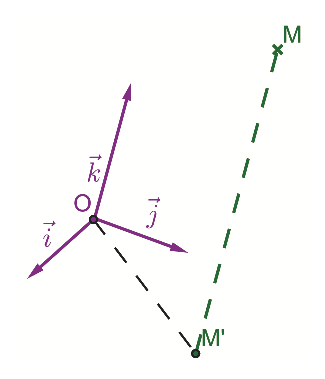
\includegraphics[width=\linewidth]{repere}\\
    \end{minipage}
  \item Unicité\\
    Supposons qu'il existe deux triplets de réels $(x\,;y\,;z)$ et
    $(x';y';z')$ tels que\\
    $ \overrightarrow{OM}=x\overrightarrow{i}+y\overrightarrow{j}+z\overrightarrow{k}=x'\overrightarrow{i}+y'\overrightarrow{j}+z'\overrightarrow{k}$.\\
    On a alors $ (z'-z)\overrightarrow{k}=(x-x')\overrightarrow{i}+(y-y')\overrightarrow{j}$.\\
    Comme $\overrightarrow{i}$, $ \overrightarrow{j}$ et
    $\overrightarrow{k}$ ne sont pas coplanaires, il n'existe pas de
    couple de réels $(\alpha;\beta)$ tels que
    $\overrightarrow{k}=\alpha\overrightarrow{i}+\beta\overrightarrow{j}$,
    on en déduit que $z-z'=0$, et par suite, que $x=x'$, $y=y'$ et
    $z=z'$.
  \end{itemize}
\end{preuve}

\begin{definition}
  $(x\,;y\,;z)$ est le triplet de coordonnées du
  point $M$ dans le repère $(O\,;\vec{i},\vec{j},\vec{k})$.

  $x$ est l'abscisse de $M$, $y$ est l'ordonnée de $M$ et $z$ est la
  cote de $M$.  

  $(x;y;z)$ sont aussi les coordonnées du vecteur
  $\overrightarrow{OM}$ dans le repère
  $(O\,;\vec{i},\vec{j},\vec{k})$.
\end{definition}
 
\begin{proprietes}
  Dans un repère $(O\ ;\vec{i},\vec{j},\vec{k})$ de l'espace,
  soit $A(x_A;y_A;z_A)$  et $B(x_B;y_B;z_B)$.  Alors :

  $\overrightarrow{AB}\begin{pmatrix}x_B-x_A\\y_B-y_A\\z_B-z_A \end{pmatrix}$

  et le milieu $K$ de $[AB]$ a pour coordonnées :   $K$
  $(\dfrac{x_A+x_B}{2};\dfrac{y_A+y_B}{2} ;\dfrac{z_A+z_B}{2})$.

  

  Si de plus $(O\ ;\ \vec{i},\vec{j},\vec{k})$ est orthonormé,
  $AB=\sqrt{(x_B-x_A)^2+(y_B-y_A)^2+(z_B-z_A)^2}$.
\end{proprietes}

\begin{proprietes}
  Dans un repère$(O\ ;\ \vec{i},\vec{j},\vec{k})$ de l'espace,
  soit $\vec{u}\begin {pmatrix} x\\y\\z \end{pmatrix}$,
  $\vec{v}\begin {pmatrix} x'\\y'\\z' \end{pmatrix}$ deux vecteurs et
  $k$ un nombre réel. Alors :

  $\vec{u}+\vec{v} \begin {pmatrix} x+x'\\y+y'\\z+z' \end{pmatrix}$ et
  $k \vec{u} \begin {pmatrix} kx\\ky\\kz \end{pmatrix}$.

  Si de plus $(O\,;\vec{i},\vec{j},\vec{k})$ est orthonormé,
  $||\vec{u}||=\sqrt{x^2+y^2+z^2}$.
\end{proprietes}

% Méthode 4 
\begin{methode}[La coplanarité  de points en utilisant leurs coordonnées]

  Il s'agit de démontrer que trois vecteurs sont coplanaires en
  écrivant l'un des vecteurs en fonction des deux autres.

  

\textbf{Exercice:}

 

  Dans un repère $(O\,;\vec{i},\vec{j},\vec{k})$ de l'espace, Démontrer
  que les points $A(1\,;2\,;0)$, $B(-1\,;1\,;1)$, $C(1\,;4\,;1)$ et $D(3\,;-1\,;-3)$
  sont coplanaires.

  

\textbf{Correction}



  $\overrightarrow{AB} 
  \begin{pmatrix} 
    -2\\
    -1\\
    \hphantom{-}1
  \end{pmatrix}$ ; $\overrightarrow{AC} \begin{pmatrix} 0\\2\\1
  \end{pmatrix}$ et $\overrightarrow{AD} \begin{pmatrix} \hphantom{-}2\\-3\\-3
  \end{pmatrix}$.

  $\overrightarrow{AB}$ et $\overrightarrow{AC}$ ne sont pas
  colinéaires, car leurs coordonnées ne sont pas proportionnelles.

  $\overrightarrow{AD}=\alpha\overrightarrow{AB}+\beta\overrightarrow{AC}\Leftrightarrow%
  \begin{cases}
    \hphantom{-}2=-2\alpha\\
    -3=-\alpha+2\beta\\
    -3=\alpha+\beta
  \end{cases}\Leftrightarrow
  \begin{cases}
    \alpha=-1\\
    \beta=-2
  \end{cases}$.

  Le système ayant un unique couple solution, les vecteurs
  $\overrightarrow{AB}$, $\overrightarrow{AC}$ et
  $\overrightarrow{AD}$ sont coplanaires, donc les points $A$, $B$,
  $C$ et $D$ sont coplanaires.
\end{methode}

\section{Représentation paramétrique de droites et de plans}

\begin{propriete}
  Dans un repère $(O\ ;\vec{i},\vec{j},\vec{k})$ de l'espace, on
  considère la droite $\mathcal{D}$ passant par $A(x_A\ ;y_A\ ;z_A)$
  et de vecteur directeur
  $\vec{u} \begin {pmatrix} \alpha\\\beta\\\gamma \end{pmatrix}$.

  $M(x;y;z)\in \mathcal{D}$ si et seulement si il existe un réel $t$
  tel que :
  \begin{center}
    $\begin{cases}x=x_A+t\alpha \\y=y_A+t\beta
      \\z=z_A+t\gamma \end{cases}$
  \end{center}
\end{propriete}

\begin{preuve}
  $M(x;y;z)\in \mathcal{D}$ si et seulement si $\overrightarrow{AM}$
  et $\vec{u}$ sont colinéaires, c'est-à-dire qu'il existe un réel $t$
  tel que $\overrightarrow{AM}=t\overrightarrow{u}$.  Cela se traduit
  en terme de coordonnées par :

  $\begin{cases}x-x_A=t\alpha \\y-y_A=t\beta
    \\z-z_A=t\gamma \end{cases}\Leftrightarrow\begin{cases}x=x_A+t\alpha
    \\y=y_A+t\beta \\z=z_A+t\gamma \end{cases}$
\end{preuve}

\begin{definition}
  On dit que le système d'équations : \\
  $\begin{cases}
    x=x_A+t\alpha    \\
    y=y_A+t\beta \\
    z=z_A+t\gamma 
  \end{cases}$
  où $t\in\mathbb{R}$ est une représentation
    paramétrique de la droite $\mathcal{D}$ passant par
  $A(x_A;y_A;z_A)$ et de vecteur directeur $\vec{u}
  \begin {pmatrix} 
    \alpha\\
    \beta\\
    \gamma 
  \end{pmatrix}$.
\end{definition}



\begin{propriete}
  Dans un  repère $(O\,;\vec{i},\vec{j},\vec{k})$  de l'espace, le plan
  $\mathcal{P}$ passant par $A(x_A;y_A;z_A)$ et de vecteurs\\ directeurs
  $\vec{u} \begin {pmatrix} \alpha\\\beta\\\gamma \end{pmatrix}$ et
  $\vec{v} \begin {pmatrix} \alpha'\\\beta'\\\gamma' \end{pmatrix}$. 

  $M(x\,;y\,;z)\in \mathcal{P}$ si et seulement si il existe deux réels
  $t$ et $t'$ tels que :
  \begin{center}
    $\begin{cases}
      x=x_A+t\alpha+t'\alpha' \\
      y=y_A+t\beta +t'\beta'  \\
      z=z_A+t\gamma +t'\gamma' 
    \end{cases}$
  \end{center}
\end{propriete}

\begin{preuve}
  $M(x\ ;\ y\ ;\ z)\in \mathcal{P}$ si et seulement si
  $\overrightarrow{AM}$, $\vec{u}$ et $\vec{v}$ sont coplanaires,
  c'est-à-dire qu'il existe deux réels $t$ et $t'$ tels que
  $\overrightarrow{AM}=t\overrightarrow{u}+t'\overrightarrow{v}$.
  Cela se traduit en terme de coordonnées par :
\begin{center}
  $\begin{cases}x-x_A=t\alpha+t'\alpha' \\
    y-y_A=t\beta +t'\beta' \\
    z-z_A=t\gamma + t'\gamma'
  \end{cases}
  \Leftrightarrow
  \begin{cases}
    x=x_A+t\alpha+t'\alpha' \\
    y=y_A+t\beta +t'\beta' \\
    z=z_A+t\gamma +t'\gamma' 
  \end{cases}$.
\end{center}
\end{preuve}

\begin{definition}
  On dit que le système d'équations :
  \\$\begin{cases}x=x_A+t\alpha+t'\alpha'
    \\y=y_A+t\beta +t'\beta' \\z=z_A+t\gamma +t'\gamma'
  \end{cases}$ où $t\in\mathbb{R}$ et
  $t'\in\mathbb{R}$
  est une représentation paramétrique du plan $\mathcal{P}$
  passant par $A(x_A\,;y_A\,;z_A)$ et de vecteurs directeurs $\vec{u}
  \begin {pmatrix} \alpha\\\beta\\\gamma \end{pmatrix}$ et
  $\vec{v} \begin {pmatrix} \alpha'\\\beta'\\\gamma' \end{pmatrix}$.
\end{definition}



\begin{remarque}
  Il existe une infinité de représentations paramétriques, que ce soit
  pour une droite ou pour un plan.
\end{remarque}

% Méthode 5
\begin{methode}[Étudier des positions relatives]

  

\textbf{Exercice:}



  

  \bgroup
  \def\columnseprule{.5pt}
  \begin{multicols}{2}
    Étudier  les positions relatives des
    droites $d$ et  $d'$ puis du plan $\wp$ et de la droite $d'$. On
    donnera leur intersection éventuelle.

    Le plan $\wp$ a pour représentation paramétrique :

    $\begin{cases} x=1-2t+3t'\\y=-2+t-t'\\z=3-t \end{cases}$ avec
    $t\in\mathbb{R}$ et $t'\in\mathbb{R}$

    

    Les droites $d$ et $d'$ ont pour représentation \mbox{paramétrique} :

    $d$ : $\begin{cases} x=2+4t\\y=5-2t\\z=1+2t \end{cases}$ avec
    $t\in\mathbb{R}$ et 

    $d'$ : $\begin{cases} x=4-t\\y=-2+t\\z=1+3t \end{cases}$ avec
    $t\in\mathbb{R}$
  \end{multicols}
  \egroup

  

\textbf{Correction}



Attention : la même lettre $t$ désigne deux paramètres différents. Il faut donc changer de lettre dans les résolutions de système pour les différencier.\\

$\wp$ est dirigé par les vecteurs $\vec{u} \begin {pmatrix} -2\\1\\-1 \end{pmatrix}$ et $\vec{v} \begin {pmatrix} 3\\-1\\-1 \end{pmatrix}$.\\
$d$ et $d'$ ont pour vecteur directeur respectif $\vec{w} \begin {pmatrix} 4\\-2\\2 \end{pmatrix}$ et $\vec{w'} \begin {pmatrix} -1\\1\\3 \end{pmatrix}$.\\
On remarque que $\overrightarrow{w}=-2\overrightarrow{u}$ donc $d$ est parallèle à $\wp$. Le point $A(2;5;1)$ appartient à $d$.
S'il appartient à $\wp$ alors $d\subset\wp$, sinon $d$ est strictement parallèle à $\wp$.\\
Or,  $\begin{cases} 2=1-2t+3t'\\5=-2+t-t'\\1=3-t \end{cases}\Leftrightarrow\begin{cases} -2t+3t'=1\\t-t'=7\\t=2 \end{cases}\Leftrightarrow\begin{cases} t'=\dfrac{5}{3}\\t'=-5\\t=2 \end{cases}$ \\
Le système n'ayant pas de solution, $A\not\in \wp$ donc $d$ est strictement parallèle à $\wp$.\\
Déterminons maintenant $\wp\cap d'$ :
$M\in\wp\cap d'\Leftrightarrow$ il existe trois réels $t$, $t'$ et $k$ tels que :\\
$\begin{cases} x=1-2t+3t'\\y=-2+t-t'\\z=3-t\\x=4-k\\y=-2+k\\z=1+3k \end{cases}\Leftrightarrow \begin{cases} 4-k=1-2t+3t'\\-2+k=-2+t-t'\\1+3k=3-t\\x=4-k\\y=-2+k\\z=1+3k \end{cases}\Leftrightarrow \begin{cases} -k+2t-3t'=-3\\k-t+t'=0\\3k+t=2\\x=4-k\\y=-2+k\\z=1+3k\end{cases}$\\
En finissant la résolution du système, on obtient 
 $t'=\dfrac{14}{5}$ ; $t=\dfrac{52}{20}$ et $k=\dfrac{-1}{5}=-0,2$, ce qui nous donne $x=4,2$ ; $y=-2,2$ et $z=0,4$.\\ 
Ainsi, $\wp$ et $d'$ sont sécantes au point $K(4,2;-2,2;0,4)$



  % \textbf{Attention :} la même lettre $t$ désigne deux paramètres
  % différents. Il faut donc changer de lettre dans les résolutions de
  % système pour les différencier.

  % $d$ et $d'$ ont pour vecteur directeur respectif $\vec{w}(4;-2;2)$
  % et $\vec{w'}(-1;1;3)$ qui ne sont pas colinéaires, donc $d$ et $d'$
  % ne sont pas parallèles.  
  % Cherchons si elles sont sécantes ou non coplanaires : 

  % Un point $M(x;y;z)$ appartient à $d$ et à $d'$ si et seulement si : 

  % $\begin{cases}
  %   2+4t=4-k\\5-2t=-2+k\\1+2t=1+3k\\x=4-k\\y=-2+k\\z=1+3k \end{cases}\Leftrightarrow \begin{cases}
  %   4t=2-k\\6=-1+4k\\2t=3k\\x=4-k\\y=-2+k\\z=1+3k \end{cases}\Leftrightarrow \begin{cases}
  %   4t=2-k\\k=\dfrac{7}{4}\\t=\dfrac{3}{2}\times\dfrac{7}{4}=\dfrac{21}{8}\\x=4-k\\y=-2+k\\z=1+3k\end{cases}\Leftrightarrow \begin{cases}
  %   t=\dfrac{1}{16}\\k=\dfrac{7}{4}\\t=\dfrac{3}{2}\times\dfrac{7}{4}=\dfrac{21}{8}\\x=4-k\\y=-2+k\\z=1+3k\end{cases}$\\Ce
  % système n'admet donc pas de solution, les droites $d$ et $d'$ sont
  % donc non coplanaires.

  % Déterminons maintenant $\wp\cap d'$ :

  % $M\in\wp\cap d'\Leftrightarrow$ il existe trois réels $t$, $t'$ et
  % $k$ tels que :

  % $\begin{cases}
  %   x=1-2t+3t'\\y=-2+t-t'\\z=3-t\\x=4-k\\y=-2+k\\z=1+3k \end{cases}\Leftrightarrow \begin{cases}
  %   4-k=1-2t+3t'\\-2+k=-2+t-t'\\1+3k=3-t\\x=4-k\\y=-2+k\\z=1+3k \end{cases}\Leftrightarrow \begin{cases}
  %   -k+2t-3t'=-3\\k-t+t'=0\\3k+t=2\\x=4-k\\y=-2+k\\z=1+3k\end{cases}$

  % $\Leftrightarrow 
  % \begin{cases} 
  %   t-2t'=-3\\
  %   3k-3t+3t'=0
  %   3k+t=2
  %   x=4-k
  %   y=-2+k
  %   z=1+3k \end{cases}\Leftrightarrow \begin{cases} 4t-8t'=-12
  %   -4t+3t'=-2
  %   2k+t=2
  %   x=4-k
  %   y=-2+k
  %   z=1+3k \end{cases}\Leftrightarrow \begin{cases}-5t'=-14
  %   4t=3t'+2
  %   2k=-t+2
  %   x=4-k
  %   y=-2+k
  %   z=1+3k \end{cases}$
  % $\Leftrightarrow \begin{cases} t'=\dfrac{14}{5}
  %   t=\dfrac{52}{20}
  %   k=\dfrac{-1}{5}=-0,2
  %   x=4,2
  %   y=-2,2
  %   z=0,4 \end{cases}$
  
  % Ainsi, $\wp$ et $d'$ sont sécantes au point $K(4,2;-2,2;0,4)$
\end{methode}

\end{document}